% ============================================================================
% AuditIQ -- camera-ready paper in the format of
% "Preparations of Papers for the Conference/Journal Publications"
% (Hinweis Research): A4; margins top/bottom 3.25 cm, left 3 cm, right 2.5 cm;
% header 1.27 cm from the top, footer 2.89 cm from the bottom; Times; title 20 pt,
% authors 10 pt, affiliations and main text 9 pt, abstract 9 pt bold, section
% titles in small capitals, subheadings 9 pt italic, tables and captions 8 pt,
% references 9 pt; no paragraph indent, no space between paragraphs; table
% captions centred above, figure captions centred below; no page numbers.
%
% Every number is taken from the result files of the repository (RESULTS.md and
% REPORT.md at https://github.com/Chandana909/major.project list each with its
% source). The propositions of Subsection V-F were checked against those files.
%
% Compile:  tectonic main.tex     (or pdflatex main.tex, twice)
% TODO before submission: add the third author's e-mail to the e-mail line.
% ============================================================================
\documentclass[9pt,a4paper,twocolumn]{extarticle}
\usepackage[T1]{fontenc}
\usepackage[a4paper,top=3.25cm,bottom=3.25cm,left=3cm,right=2.5cm,columnsep=0.5cm,
            headheight=12pt,headsep=1.56cm,footskip=0.36cm]{geometry}
\usepackage{times}
\usepackage{amsmath,amssymb,amsthm}
\usepackage{booktabs,array}
\usepackage{caption}
\usepackage{titlesec}
\usepackage{algorithm}
\usepackage{algpseudocode}
\usepackage{tikz}
\usetikzlibrary{arrows.meta,positioning}
\usepackage{pgfplots}
\pgfplotsset{compat=1.18}
\usepackage{url}
\usepackage[hidelinks]{hyperref}
\usepackage{balance}

% ---- page and paragraphs ----------------------------------------------------
\pagestyle{empty}                                  % no page numbers
\setlength{\parindent}{0pt}                        % no indent
\setlength{\parskip}{0pt}                          % no space between paragraphs
\renewcommand{\baselinestretch}{1.0}               % single spaced
\setlength{\abovedisplayskip}{6pt}\setlength{\belowdisplayskip}{6pt}
\setlength{\abovedisplayshortskip}{6pt}\setlength{\belowdisplayshortskip}{6pt}

% ---- headings ---------------------------------------------------------------
\newcommand{\twospaces}{\hspace{2\fontdimen2\font}}
\renewcommand{\thesection}{\Roman{section}}
\renewcommand{\thesubsection}{\thesection-\Alph{subsection}}
\titleformat{\section}{\centering\fontsize{9}{11}\selectfont\scshape}{\thesection.\twospaces}{0pt}{}
\titlespacing*{\section}{0pt}{12pt}{6pt}
\titleformat{\subsection}{\fontsize{9}{11}\selectfont\itshape}{\Alph{subsection}.\twospaces}{0pt}{}
\titlespacing*{\subsection}{0pt}{6pt}{3pt}

% ---- captions: 8 pt; TABLE I. above, centred; Fig. 1. below, centred ---------
\DeclareCaptionFont{eight}{\fontsize{8}{9.5}\selectfont}
\DeclareCaptionTextFormat{upper}{\MakeUppercase{#1}}
\captionsetup{font=eight,labelsep=period,justification=centering,singlelinecheck=false}
\captionsetup[table]{name=TABLE,textformat=upper,position=top,skip=3pt}
\captionsetup[figure]{name=Fig.,skip=4pt}
\renewcommand{\thetable}{\Roman{table}}
\newcommand{\tablefont}{\fontsize{8}{9.5}\selectfont}

% ---- theorems ---------------------------------------------------------------
\newtheorem{proposition}{Proposition}
\newtheorem{definition}{Definition}
\newcommand{\Vc}{V^{\mathrm{c}}}
\newcommand{\rp}{\hat{\theta}}
\algrenewcommand\algorithmicrequire{\textbf{Input:}}
\algrenewcommand\algorithmicensure{\textbf{Output:}}
\newcolumntype{L}[1]{>{\raggedright\arraybackslash}p{#1}}

% ---- references: 9 pt ------------------------------------------------------
\makeatletter
\renewcommand\@biblabel[1]{[#1]}
\makeatother

\begin{document}

\twocolumn[{%
\begin{center}
\vspace*{6pt}
{\fontsize{20}{24}\selectfont A Distributed Multi-Agent AI Platform for Scalable\\ Forensic Audit and Compliance\par}
\vspace{6pt}
{\fontsize{10}{12}\selectfont Podichetty Samiksha\textsuperscript{1}, Chandana Devanaboyina\textsuperscript{2} and Medapally Shiva Reddy\textsuperscript{3}\par}
\vspace{3pt}
{\fontsize{9}{11}\selectfont
\textsuperscript{1--3}Department of Information Technology, Chaitanya Bharathi Institute of Technology, Hyderabad, India\\
Email: samiksha10.1b@gmail.com, chandanad3884@gmail.com\par}
\end{center}
\vspace{6pt}
{\fontsize{9}{11}\selectfont\bfseries
\textit{Abstract}---Procurement audit tests every invoice against its order, receipt, vendor and approval records, and justifies each exception against a written policy. Large language models (LLMs) can read such policies, yet they detect errors while rarely citing the governing rule, and policy thresholds drift silently out of the prompts and code meant to enforce them. We present a distributed multi-agent platform for forensic audit whose central contribution is a policy compiler: the policy document is parsed into a typed clause registry that twelve deterministic controls execute before any LLM is invoked, so that no threshold resides in code or prompts and no model can retract a decidable finding. We formalise threshold drift and show that an auditor with frozen thresholds errs on exactly the displaced decisions, with a polarity fixed by the direction of the change. On synthetic ledgers of 40{,}000 invoices, the compiler recovered 196 of 196 thresholds from fourteen documents and 280 of 280 from twenty held-out ones; the controls made no wrong decision in 1{,}360{,}000 audits, whereas frozen thresholds misdecided up to 30.7\% of invoices. On three benchmark ledgers the controls reached an F1 of 0.833 at a precision of 1.000, against 0.536 and 0.498 for an isolation forest and a one-class SVM, at under 20\,$\mu$s per invoice. On a 34-invoice sample, agents using a local 7B model found 12 of 20 judgement anomalies, but only 0.375 of their findings named the violated rule. All data are synthetic.

\vspace{6pt}
\textit{Index Terms}---forensic audit, multi-agent systems, large language models, policy as data, deterministic controls, threshold drift.\par}
\vspace{12pt}
}]

% ============================================================================
\section{Introduction}
An auditor who tests procurement spend must establish, for every invoice, that it corresponds to an approved purchase order (PO), that the goods or services were received (goods receipt note, GRN), that the vendor is legitimate and tax-compliant, and that the payment was approved within the approver's delegated limit. The evidence is scattered across records, and what counts as an exception is fixed by an organisation-specific policy. Continuous auditing proposes to test every transaction rather than a sample [1].

Large language models (LLMs) are a natural candidate for this work, because the policy is written in prose. AuditBench [2] delineates their limits: given transaction histories, LLMs identify errors, but explain them poorly and rarely cite the relevant standard. Systems of cooperating, specialised LLM agents are increasingly proposed for financial tasks [3]. Building such a pipeline exposed a second, structural problem, which we call the \emph{policy--implementation gap}: tolerances and limits were stated in prose, one of them was duplicated as a literal in an agent prompt, and whether a rule was checked at all depended on an agent electing to call a tool. Every revision of the policy demanded a manual edit of the system, with no evidence that the edit matched the document.

This paper presents a distributed multi-agent platform for forensic audit in procurement. \emph{Forensic} means that every decision is reconstructible: each finding carries its rule, its evidence and the page of the policy it rests on, and every stage appends to an audit trail. \emph{Distributed} means that the platform is a set of separable services communicating over network interfaces. We retain the base pipeline of [2], [3] and close the gap with one feature. Our contributions are:
\begin{enumerate}\setlength{\itemsep}{0pt}\setlength{\parsep}{0pt}\setlength{\topsep}{2pt}
\item a \emph{policy compiler} that turns the policy document into an executable clause registry, with explicit refusal semantics for documents it cannot execute (Subsection~\ref{sec:compiler});
\item a controls-first architecture with a \emph{non-interference} guarantee: no LLM stage can retract or weaken a deterministic finding (Proposition~\ref{prop:ni});
\item a formal account of \emph{threshold drift}: the error of a frozen auditor equals the decision displacement of the policy change, and its polarity is fixed by the direction of the change (Propositions~\ref{prop:drift} and~\ref{prop:polarity}), confirmed on 34 policy variants;
\item a comparison with two classical anomaly detectors and an end-to-end evaluation of the LLM stages, with an open, reproducible artefact.
\end{enumerate}

% ============================================================================
\section{Base Papers}
\subsection{AuditBench}
Wang et al. [2] pair financial tables with synthetic transactions into which errors are injected, and evaluate LLMs on financial-statement audit. Their finding that LLMs detect errors but explain them and cite the governing standard poorly is the reason our findings must name the rule they rely on. We adopt their construction of evaluation data with injected, labelled errors, and their requirement that a finding cite its rule. AuditBench measures models; it does not propose a system that removes the weakness, nor does it address procurement documents checked against an organisation's own policy.

\subsection{LLM-Based Multi-Agent Systems in Finance}
Liu et al. [3] survey LLM-based multi-agent systems for financial markets and argue that agents which are heterogeneous, autonomous and boundedly rational suit markets better than traditional models. We adopt the architecture of specialist agents with their own roles and views of the data, whose outputs are combined. The survey concerns market simulation rather than audit, and names regulatory traceability of agent decisions as an open challenge, which an audit system must answer concretely.

% ============================================================================
\section{Related Work}
\subsection{Anomaly Detection}
Anomaly detection ranks records by how unusual they are [4]; statistical fraud detection has long been reviewed [5]. Isolation forests [6] and one-class support vector machines (SVMs) [7] are standard unsupervised choices, and we use both as baselines. A detector returns a score, not a rule: an unusual record need not violate policy, a violation (an invoice approved above a delegated limit) need not look unusual, and a policy change requires retraining.

\subsection{LLMs in Audit and Compliance}
LLMs have matched financial text against audit requirements [8] and verified the regulatory compliance of financial reports [9]. Generated text can assert facts the input does not support [10], which an audit cannot accept. Retrieval-augmented generation [11] grounds answers in retrieved passages, as our copilot does, but grounding alone does not make a rule citation correct.

\subsection{Multi-Agent LLM Systems}
Surveys of LLM-based agents are given in [12]; debate between agents improves factual accuracy [13]; review of uncertain cases by a human remains the accepted safeguard for high-stakes decisions [14].

\subsection{Research Gap}
Prior work either detects anomalies without naming a rule or lets an LLM reason over the policy text. To our knowledge, no published work lets the policy document itself configure executable audit controls, so that the thresholds a system applies are provably those the document states.

% ============================================================================
\section{Problem Formulation}
\label{sec:formal}
A ledger is a set $\mathcal{L}=\{x_1,\dots,x_N\}$ of transactions. A transaction $x$ is an invoice together with its PO, its GRN, the vendor master record, the approval-log entries and the vendor's other invoices.

\begin{definition}[Policy]
A policy version is a tuple $P=(K,s,\kappa,\theta)$: a set $K$ of rule identifiers; a severity $s:K\to\{\mathrm{critical},\mathrm{high},\mathrm{medium},\mathrm{low}\}$; a kind $\kappa:K\to\{\mathrm{control},\mathrm{judgement}\}$, stating whether a rule is decidable by comparing fields; and parameters $\theta=(\theta_k)_{k\in K}$. We write $K_c=\{k:\kappa(k)=\mathrm{control}\}$.
\end{definition}

Our reference policy (version 2.5) has $|K|=16$ rules, $|K_c|=12$, and 14 parameter values. Let $V_P(x)\subseteq K$ be the rules that $x$ violates under $P$, computed by an independent validator, and $\Vc_P(x)=V_P(x)\cap K_c$. An auditor $\mathcal{A}$ cites a set $C_{\mathcal{A}}(x)$ of rules.

\begin{definition}[Adherence and Displacement]
The adherence of $\mathcal{A}$ to $P$ is
\begin{equation}
\mathrm{A}_P(\mathcal{A})=\frac{1}{N}\sum_{x\in\mathcal{L}}\mathbf{1}\bigl[C_{\mathcal{A}}(x)=\Vc_P(x)\bigr].
\label{eq:adherence}
\end{equation}
The decision displacement of a change from $P_0$ to $P$ is $\Delta(P_0,P)=\{x\in\mathcal{L}:\Vc_P(x)\neq\Vc_{P_0}(x)\}$.
\end{definition}

The \emph{policy-driven} auditor executes the controls under parameters $\rp=E(D)$ extracted from the document $D$ of $P$; the \emph{frozen} auditor executes the same controls under the parameters $\theta_0$ of $P_0$, which models a system whose thresholds are written into prompts and code until someone edits them.

% ============================================================================
\section{Proposed System}
\label{sec:system}
\subsection{Architecture}
The platform comprises audit workers, a policy service, a relational data store (SQLite or PostgreSQL), a model endpoint with an OpenAI-compatible interface, and a representational state transfer (REST) application programming interface (API) with a web application for reviewers (Fig.~\ref{fig:arch}). One invoice is one unit of work: its transaction carries every record it needs, so workers require no coordination. The pipeline is a LangGraph [15] state graph: evidence extraction, deterministic controls, three specialist agents in parallel (math and approvals; tax and identity; vendor intelligence), a challenger, a confidence stage, risk scoring and routing, and human review with an audit pack. Each agent sees only the records its rules need, and a finding that cites a rule outside its remit is discarded by code. Results are appended, never replaced.

\begin{figure*}[t]
\centering
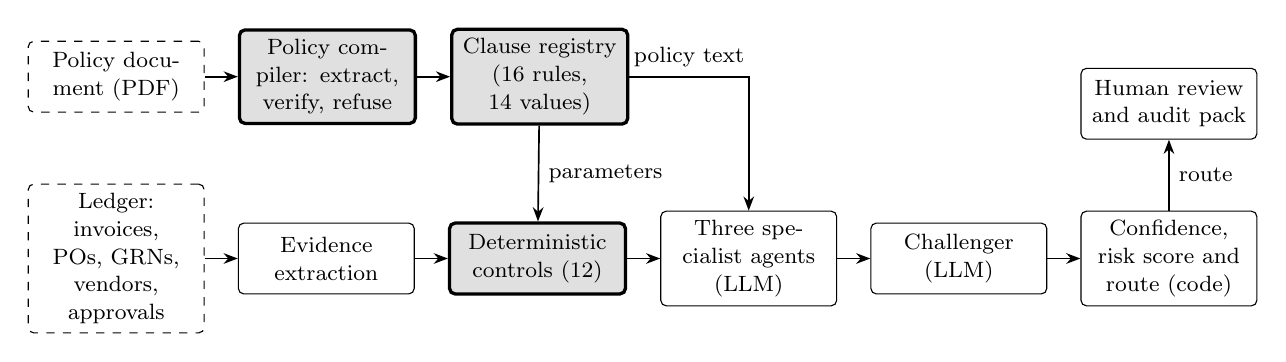
\begin{tikzpicture}[font=\fontsize{8.5}{10}\selectfont, node distance=4mm and 4.2mm,
  base/.style={draw, rounded corners=2pt, minimum height=9mm, text width=20mm, align=center, fill=white},
  new/.style={draw, very thick, rounded corners=2pt, minimum height=9mm, text width=20mm, align=center, fill=black!12},
  data/.style={draw, dashed, rounded corners=2pt, minimum height=9mm, text width=20mm, align=center},
  arr/.style={-{Stealth[length=1.8mm]}, semithick}]
\node[data] (pdf) {Policy document (PDF)};
\node[new, right=of pdf] (comp) {Policy compiler: extract, verify, refuse};
\node[new, right=of comp] (reg) {Clause registry (16 rules, 14 values)};
\node[data, below=9mm of pdf] (led) {Ledger: invoices, POs, GRNs, vendors, approvals};
\node[base, right=of led] (ext) {Evidence extraction};
\node[new, right=of ext] (ctl) {Deterministic controls (12)};
\node[base, right=of ctl] (agt) {Three specialist agents (LLM)};
\node[base, right=of agt] (chl) {Challenger (LLM)};
\node[base, right=of chl] (scr) {Confidence, risk score and route (code)};
\node[base, above=9mm of scr] (rev) {Human review and audit pack};
\draw[arr] (pdf) -- (comp);
\draw[arr] (comp) -- (reg);
\draw[arr] (led) -- (ext);
\draw[arr] (ext) -- (ctl);
\draw[arr] (ctl) -- (agt);
\draw[arr] (agt) -- (chl);
\draw[arr] (chl) -- (scr);
\draw[arr] (scr) -- node[right] {route} (rev);
\draw[arr] (reg) -- node[right] {parameters} (ctl);
\draw[arr] (reg.east) -| node[pos=0.25, above] {policy text} (agt.north);
\end{tikzpicture}
\caption{The proposed system. Grey boxes with a thick border are the extra feature, white boxes the base pipeline and dashed boxes data. The policy document configures the controls, which run before any LLM is called; scoring and routing are code.}
\label{fig:arch}
\end{figure*}

\subsection{Policy Compilation}
\label{sec:compiler}
The compiler (Algorithm~\ref{alg:compile}) reads every text line of the portable document format (PDF) file with its font size, position and page, and segments the text into numbered rules by layout rather than keyword: the modal font size is the body size, a line at least one point larger is a heading, and a line opening with ``Rule $\langle$number$\rangle$ ($\langle$severity$\rangle$),'' starts a rule. One pattern per parameter is matched against the wording of the rule that states it; approval limits are read from the table of roles. No language model participates: a value is either found in its sentence or reported missing. The rule set $K$ and the kinds $\kappa$ come from a reference version, which records what the system can execute.

\begin{algorithm}[t]
\caption{Policy compilation with refusal}
\label{alg:compile}
\fontsize{8}{9.5}\selectfont
\begin{algorithmic}[1]
\Require policy PDF $D$; reference policy $P_{\mathrm{ref}}=(K,s,\kappa,\theta_{\mathrm{ref}})$
\Ensure registry $\hat{P}$ or a list $\Pi$ of problems
\State $\Lambda\gets$ text lines of $D$ with font size, position, page
\State $\mathcal{R}\gets$ rules segmented from $\Lambda$ by layout; $\Pi\gets\emptyset$
\ForAll{$k\in K$}
  \If{$k\notin\mathcal{R}$} $\Pi\gets\Pi\cup\{$``rule $k$ absent''$\}$
  \ElsIf{$k$ stated more than once} $\Pi\gets\Pi\cup\{$``$k$ ambiguous''$\}$
  \Else\ $\hat{s}(k)\gets$ severity stated in $\mathcal{R}_k$
    \ForAll{parameter $p$ of $k$}
      \State $\hat{\theta}_{k,p}\gets$ match the pattern of $p$ in $\mathcal{R}_k$
      \If{no match or value not meaningful} $\Pi\gets\Pi\cup\{(k,p)\}$ \EndIf
    \EndFor
  \EndIf
\EndFor
\State add to $\Pi$: rules in $\mathcal{R}\setminus K$; no version; approval table missing a role
\If{$\Pi\neq\emptyset$} \Return $\Pi$ \Comment{refused; nothing stored} \EndIf
\State \Return $\hat{P}=(K,\hat{s},\kappa,\hat{\theta})$ with passages and pages
\end{algorithmic}
\end{algorithm}

\subsection{Deterministic Controls}
A control $c_k(x;\theta_k)$ is a pure function of a transaction and the parameters of its rule. It returns nothing or a finding $f=(k,s(k),E)$, where $E$ is the set of field values it rests on; when the result is stored, the finding is attached to the document and page of its rule. A control contains no constant of its own. For example, the amount-match control raises a finding if and only if
\begin{equation}
100\,\lvert a_{\mathrm{inv}}-a_{\mathrm{po}}\rvert>\hat{\theta}_{2.1.1}\,a_{\mathrm{po}},
\label{eq:amount}
\end{equation}
where $a_{\mathrm{inv}}$ and $a_{\mathrm{po}}$ are the invoice and PO amounts in integer paise, so that rounding cannot move a decision at the boundary, and $\hat{\theta}_{2.1.1}$ is the tolerance in percent read from the document. The approval-limit control takes the limit of the approving role from the registry, not from the approval log, because the log records what the approval system believed at the time. The controls run as $F_D(x)=\{c_k(x;\rp_k):k\in K_c\}$.

\subsection{Agentic Layer}
The four judgement rules (receipt remarks, description match, near-duplicates, structuring across days) are assigned to three specialist agents whose remits follow the sections of the policy. Prompts contain no threshold and no rule number; the policy text is inserted at run time. The challenger, in the spirit of multi-agent debate [13], may remove agent findings that the evidence does not support. In configuration C5, the full pipeline (configurations C1 to C5 are defined in Subsection~\ref{sec:llmsetup}), each model finding $f$ receives a confidence
\begin{equation}
c(f)=\tfrac{1}{3}\bigl(g(f)+p(f)+a(f)\bigr),
\label{eq:conf}
\end{equation}
where $g=1$ if every evidence field exists in the transaction with the stated value, $p=1$ if the cited rule exists in the active policy, and $a$ is the share of $m=3$ re-runs at temperature 0.7 that cite the same rule; $c(f)=1$ for a control finding.

\subsection{Risk Scoring and Routing}
With weights $w=(30,20,10,5)$ for critical, high, medium and low findings, the count-based and confidence-weighted scores are
\begin{align}
R_0(x)&=\min\Bigl(100,\textstyle\sum_{f\in F(x)}w_{s(f)}\Bigr),\label{eq:r0}\\
R_c(x)&=\min\Bigl(100,\textstyle\sum_{f\in F(x)}w_{s(f)}\,c(f)\Bigr),\label{eq:rc}
\end{align}
each raised to at least 70 (50) by a critical (high) finding, for $R_c$ only by findings with $c(f)\ge\vartheta=2/3$. An invoice is escalated if $R_c\ge\tau=50$, sent to sampled review if $R_c<\tau\le R_0$, and approved otherwise.

\subsection{Formal Properties}
\begin{proposition}[Non-Interference]\label{prop:ni}
In every configuration with controls, $F_D(x)\subseteq F(x)$ and each $f\in F_D(x)$ enters (\ref{eq:r0}) and (\ref{eq:rc}) with $c(f)=1$. Hence $R_c(x)\ge R_0^{\mathrm{C1}}(x)$, and every invoice escalated by the controls alone remains escalated whatever the LLM stages output.
\end{proposition}
\begin{proof}[Sketch]
The challenger's action space is restricted to agent findings, and model findings add non-negative terms to (\ref{eq:rc}); the floors triggered by control findings are unaffected. \qedhere
\end{proof}

\begin{proposition}[Drift Identity]\label{prop:drift}
If the controls are faithful under $P_0$, that is $C(x)=\Vc_{P_0}(x)$ for all $x$, then the frozen auditor satisfies $\mathrm{A}_P(\mathrm{frozen})=1-\lvert\Delta(P_0,P)\rvert/N$.
\end{proposition}
\begin{proof}[Sketch]
The frozen auditor cites $\Vc_{P_0}(x)$, which equals $\Vc_P(x)$ if and only if $x\notin\Delta(P_0,P)$. \qedhere
\end{proof}

\begin{proposition}[Error Polarity]\label{prop:polarity}
If a change tightens the policy, $\Vc_{P_0}(x)\subseteq\Vc_P(x)$ for all $x$, every error of the frozen auditor is an omission (a missed exception); if it loosens the policy, $\Vc_{P_0}(x)\supseteq\Vc_P(x)$, every error is a commission (an unsupported finding).
\end{proposition}
\begin{proof}[Sketch]
Errors are $\Vc_P\setminus\Vc_{P_0}$ (omissions) and $\Vc_{P_0}\setminus\Vc_P$ (commissions); one of the two is empty under each inclusion. For threshold rules the inclusion follows from the order of the parameter: a smaller tolerance, a lower daily count or approval limit, a superset of non-business days or blocked statuses, or a divisor of the round-amount multiple tightens. \qedhere
\end{proof}

Propositions~\ref{prop:drift} and~\ref{prop:polarity} make the error of the frozen system a property of the ledger and the change, not of the implementation; Section~\ref{sec:results} measures it.

% ============================================================================
\section{Experimental Setup}
\subsection{Data}
All data are synthetic. Following AuditBench [2], anomalies are injected into synthetic transactions and labelled when injected; an independent validator, sharing no code with the controls, recomputes $V_P$ from the finished tables and rejects any ledger whose labels it does not reproduce. Three benchmark ledgers of 5{,}000 invoices hold 420 anomalous invoices (8.4\%) in fourteen classes, ten rule-defined and four judgement classes, and 120 hard negatives: clean invoices built to resemble an anomaly. A 20{,}000-invoice ledger holds 420 anomalous invoices of the same composition (2.1\%). Five ledgers of 40{,}000 invoices in total carry the policy experiments.

\subsection{Policies}
From version 2.5 we derive fourteen variants (eleven change one threshold, three change several), twenty further variants drawn at random with a fixed seed from value ranges never used to build or test the compiler, and sixteen edited copies of the reference document that test refusal. Each is rendered as a PDF file, the only input the system receives.

\subsection{Baselines}
An isolation forest [6] (300 trees, fitted without labels on all invoices) and a one-class SVM [7] (radial basis function kernel, $\nu=0.1$, fitted on the clean invoices of the training folds), both from scikit-learn [16], on 21 generic features that encode no policy threshold. Thresholds are set by five-fold cross-fitting, stratified by class: each fold is decided with the threshold that maximises F1 on the other four, so no invoice is decided with a threshold tuned on its own label. As a detector names no rule, an invoice counts as detected when reported at all.

\subsection{LLM Stages}
\label{sec:llmsetup}
Qwen2.5-7B [17] served locally on a laptop central processing unit (CPU), temperature 0. Configurations: C1, controls alone; C2, one prompt over the whole policy, no controls; C3, controls and three agents; C4, C3 with the challenger; C5, C4 with confidence. Prompts were tuned only on a development ledger and frozen before evaluation (one prompt hash across all runs). We evaluate on 20 invoices of the development ledger (one per anomaly class, one per hard-negative type, one ordinary) and on a 34-invoice sample of benchmark ledger 101 (five per judgement class, two per hard-negative type, four ordinary).

\subsection{Statistics}
We report 95\% percentile bootstrap intervals over invoices (1{,}000 resamples) and McNemar's exact test on paired per-invoice correctness, with Holm's adjustment.

% ============================================================================
\section{Results}
\label{sec:results}
\subsection{Compilation Fidelity}
The compiler accepted all fourteen variants and recovered 196 of 196 parameter values and 224 of 224 rules word for word, in 0.01--0.09\,s per document. On the twenty held-out variants it recovered 280 of 280 values and 320 of 320 rules. Of the sixteen edited documents, all seven that preserve every value were read correctly and all seven that make the document unexecutable were refused with a reason. The two ambiguous documents, a rule stated twice with two values and an approval table lacking a role, were adopted in a first run; both checks were added with regression tests, after which all sixteen were handled as required.

\subsection{Adherence and Threshold Drift}
Table~\ref{tab:drift} reports every one of the fourteen variants. The policy-driven controls decided every invoice as the policy in force requires: no wrong decision in 560{,}000 audits over the fourteen variants and 800{,}000 over the twenty held-out variants. Under version 2.5 the controls and the validator agree on 40{,}000 of 40{,}000 invoices, so Proposition~\ref{prop:drift} applies; indeed the errors of the frozen auditor equal the decision displacement in all 34 variants. Displacement ranges from none to 12{,}274 invoices (30.7\%) over the fourteen variants and up to 7{,}953 (19.9\%, median 79) over the held-out ones. Polarity behaves as Proposition~\ref{prop:polarity} predicts: each of the fourteen variants produces errors of a single polarity. The five tightening variants cause 24{,}854 missed exceptions and 24{,}177 missed escalations, a silent failure; the eight loosening variants cause 1{,}069 unsupported findings and 913 needless escalations, a cost in reviewer time. Each of the five held-out variants with both polarities combines a tightening and a loosening component, such as replacing Sunday by Friday as a non-business day.

\begin{table*}[t]
\caption{Policy Change: Adherence to the Policy in Force on 40{,}000 Invoices per Policy}
\label{tab:drift}
\centering\tablefont\setlength{\tabcolsep}{6pt}
\begin{tabular}{lrrrrrrr}
\toprule
 & Displaced & \multicolumn{2}{c}{Adherence} & \multicolumn{2}{c}{Frozen: omissions} & \multicolumn{2}{c}{Frozen: commissions}\\
\cmidrule(lr){3-4}\cmidrule(lr){5-6}\cmidrule(lr){7-8}
Policy variant (new value) & invoices & driven & frozen & exceptions & escalations & findings & escalations\\
\midrule
Tolerance 0.5\% & 62 & 1.000 & 0.998 & 62 & 62 & 0 & 0 \\
Tolerance 2\% & 7 & 1.000 & 1.000 & 0 & 0 & 7 & 7 \\
Tolerance 5\% & 63 & 1.000 & 0.998 & 0 & 0 & 63 & 63 \\
Daily count 2 & 429 & 1.000 & 0.989 & 429 & 428 & 0 & 0 \\
Daily count 5 & 170 & 1.000 & 0.996 & 0 & 0 & 170 & 170 \\
Manager limit 50,000 & 7{,}677 & 1.000 & 0.808 & 7{,}677 & 7{,}514 & 0 & 0 \\
Manager limit 150,000 & 69 & 1.000 & 0.998 & 0 & 0 & 69 & 69 \\
Senior Manager limit 250,000 & 4{,}259 & 1.000 & 0.894 & 4{,}259 & 4{,}161 & 0 & 0 \\
Round multiple 5,000 & 0 & 1.000 & 1.000 & 0 & 0 & 0 & 0 \\
Round multiple 50,000 & 43 & 1.000 & 0.999 & 0 & 0 & 43 & 0 \\
Six-day week & 35 & 1.000 & 0.999 & 0 & 0 & 35 & 0 \\
Strict policy & 12{,}274 & 1.000 & 0.693 & 12{,}427 & 12{,}012 & 0 & 0 \\
Lenient policy & 380 & 1.000 & 0.991 & 0 & 0 & 380 & 302 \\
Version 2.6 & 302 & 1.000 & 0.992 & 0 & 0 & 302 & 302 \\
\bottomrule
\end{tabular}

\vspace{3pt}\parbox{0.92\textwidth}{\fontsize{7}{8.5}\selectfont Reference version 2.5: tolerance 1\%, daily count 3, Manager limit 100{,}000, Senior Manager limit 500{,}000, round multiple 10{,}000, Saturday and Sunday non-business days. Strict policy: tolerance 0.5\%, daily count 2, Manager 50,000, Senior Manager 250,000, round multiple 5,000. Lenient policy: tolerance 5\%, daily count 5, Manager 150,000, six-day week, round multiple 50,000. Version 2.6: tolerance 5\%, daily count 5, Manager 150,000. Omissions: exceptions the policy requires that the frozen auditor does not raise, and invoices it approves although the policy sends them to review. Commissions: findings the policy no longer supports, and invoices escalated needlessly. Exceptions and findings count rules; the other columns count invoices.}
\end{table*}

\subsection{Detection Against Classical Detectors}
Table~\ref{tab:detect} compares the controls with the detectors. The controls attain the highest recall and F1 at a precision of 1.000 and raise no finding on any clean invoice, hard negatives included, whereas the detectors flag 36\% to 56\% of the hard negatives across the benchmark ledgers (their false-positive rate, FPR). McNemar's test favours the controls over each detector on every benchmark ledger (Holm-adjusted $p<10^{-50}$). At the realistic anomaly rate of the 20{,}000-invoice ledger, the isolation forest falls to an F1 of 0.211 and the one-class SVM to 0.429, while the controls keep 0.833. The recall of 1.000 of the controls on the ten rule-defined classes is by construction, since they implement the definitions by which those anomalies were injected; the behaviour of the detectors is not. Strikingly, a single binary feature, whether the Goods and Services Tax Identification Number (GSTIN) on the invoice differs from the registered one, separates the two GSTIN classes from every ordinary invoice (on ledger 101, 30 of 30 invoices per class against 0 of 4{,}460), yet the one-class SVM reports on average only 3.3\% of them. Both detectors find the near-duplicates (J1) that the controls leave to the agents, but name no rule.

\begin{table}[t]
\caption{Invoice-Level Detection: Mean of Three Benchmark Ledgers (5{,}000 Invoices, 8.4\% Anomalous)}
\label{tab:detect}
\centering\tablefont\setlength{\tabcolsep}{4pt}
\begin{tabular}{L{2.9cm}rrr}
\toprule
Measure & Isolation & One-class & Controls\\
 & forest & SVM & \\
\midrule
Recall & 0.577 & 0.464 & 0.714 \\
Precision & 0.501 & 0.543 & 1.000 \\
F1 & 0.536 & 0.498 & 0.833 \\
FPR, hard negatives & 0.403 & 0.481 & 0.000 \\
FPR, ordinary invoices & 0.044 & 0.025 & 0.000 \\
F1 on the 20{,}000-invoice ledger (2.1\% anomalous) & 0.211 & 0.429 & 0.833 \\
\bottomrule
\end{tabular}
\end{table}

\subsection{Throughput}
The control stage costs 17.8--19.4\,$\mu$s per invoice in one process, independently of ledger size between 5{,}000 and 40{,}000 invoices, so its cost is linear in the ledger. Because invoices are independent units of work, the stage parallelises without coordination (Fig.~\ref{fig:scal}): on 300{,}000 invoice audits, throughput rose from 56{,}660 invoices per second with one worker to 172{,}226 with eight (speed-up 3.04 on 2 performance and 8 efficiency cores), every configuration producing the same 16{,}840 findings. With every result, finding and trail entry stored, one process audits 20{,}000 invoices in under a minute.

\begin{figure}[t]
\centering
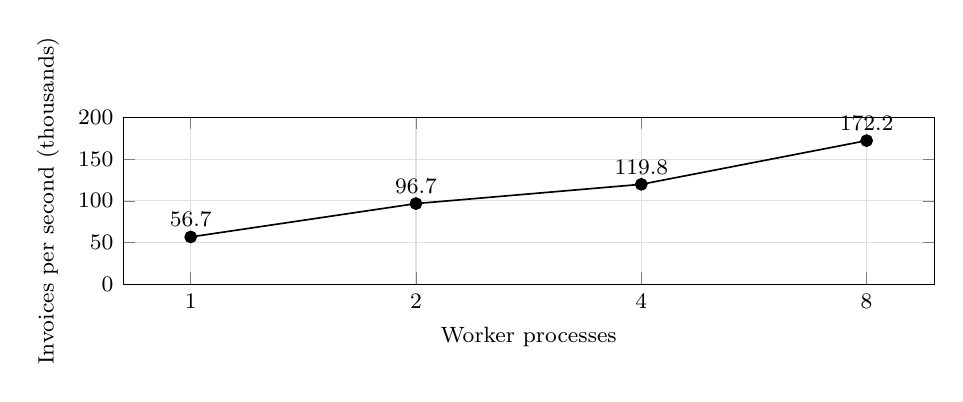
\begin{tikzpicture}
\begin{axis}[width=0.98\columnwidth, height=3.7cm, xmode=log, log basis x=2,
  xtick={1,2,4,8}, xticklabels={1,2,4,8}, ymin=0, ymax=200,
  xlabel={Worker processes}, ylabel={Invoices per second (thousands)},
  label style={font=\fontsize{8.5}{10}\selectfont}, tick label style={font=\fontsize{8}{9}\selectfont},
  nodes near coords, nodes near coords style={font=\fontsize{8}{9}\selectfont, color=black},
  grid=major, grid style={black!12}]
\addplot[color=black, mark=*, semithick] coordinates {(1,56.7) (2,96.7) (4,119.8) (8,172.2)};
\end{axis}
\end{tikzpicture}
\caption{Throughput of the control stage on one laptop (median of three runs).}
\label{fig:scal}
\end{figure}

\subsection{The LLM Stages}
Table~\ref{tab:llm} summarises the 34-invoice sample. The controls alone find none of the 20 judgement anomalies, by design. The agents of C3 found 12: all five near-duplicates, four of five goods-receipt remarks, two of five cross-day structuring cases and one of five description mismatches; yet only 0.375 of their 32 findings named a violated rule. The single prompt of C2 found 4, flagged seven of ten hard negatives and all four ordinary invoices, and named a violated rule in 0.031 of its 128 findings. The challenger of C4 halved the false alarms on hard negatives (eight to four) and raised the share of findings naming a violated rule to 0.471, but removed four of the five correct near-duplicate findings. C5 sent four invoices to sampled review, three of them true anomalies. Agreement over re-runs did not separate right from wrong: 6 of 9 wrong and 5 of 8 right model findings kept by C5 had full agreement. On the 20-invoice pilot, every rule-defined class was decided correctly with the controls first and, as Proposition~\ref{prop:ni} requires, all ten control findings and all eight control escalations survived C3--C5 unchanged. No difference between configurations is significant (C3 against C2, $p=0.277$).

\begin{table}[t]
\caption{LLM Configurations on the 34-Invoice Sample (Qwen2.5-7B)}
\label{tab:llm}
\centering\tablefont\setlength{\tabcolsep}{3.4pt}
\begin{tabular}{L{3.2cm}rrrr}
\toprule
Measure & C2 & C3 & C4 & C5\\
\midrule
Judgement anomalies found (of 20) & 4 & 12 & 8 & 8 \\
Hard negatives flagged (of 10) & 7 & 8 & 4 & 4 \\
Ordinary invoices flagged (of 4) & 4 & 3 & 2 & 2 \\
Findings naming a violated rule & 0.031 & 0.375 & 0.471 & 0.471 \\
Sent to sampled review & -- & -- & -- & 4 \\
Model calls per invoice & 1.21 & 3.00 & 3.74 & 5.24 \\
\bottomrule
\end{tabular}
\end{table}

% ============================================================================
\section{Discussion}
The adherence of 1.000 certifies the mechanism, not the rules: the controls and the validator are two implementations of the same written rules, and their agreement shows that each document was compiled correctly and that no control harbours a threshold of its own. The substantive quantities are those of the frozen auditor. By Proposition~\ref{prop:drift} its error is the displacement of the change, and ordinary revisions of a procurement policy displace between none and almost a third of the decisions on these ledgers; by Proposition~\ref{prop:polarity}, a frozen system fails silently under every tightening.

For the twelve decidable rules, the citation failure that AuditBench reports cannot arise: a finding is bound to its rule by the control that implements it. For the four judgement rules, the low share of agent findings that name a violated rule reproduces that failure, and neither the challenger nor agreement-based confidence removes it; this is why those rules remain under human review. The architecture thus does not solve the unreliability of LLMs; it \emph{confines} it, moving every decidable rule out of the reach of the model (Proposition~\ref{prop:ni}) and leaving the errors of the model where a reviewer can see them.

% ============================================================================
\section{Limitations}
\subsection{Synthetic Data}
All ledgers are synthetic; the counts describe how these ledgers react to these changes, not the books of an organisation.

\subsection{Circularity}
The controls and the ground truth implement the same written rules; perfect scores on the rule-defined classes verify the implementation, not that the rules catch real fraud.

\subsection{LLM Evaluation}
The LLM stages were measured on 20 and 34 invoices with one 7B model on a laptop CPU; the samples are too small to separate configurations, and accuracy on whole benchmark ledgers is unmeasured.

\subsection{Compiler Scope and Deployment}
Pattern extraction reads one template's wording and refuses other documents with reasons; a model-assisted path for documents in their own wording proposed 80 of 84 values correctly on six short documents, but two wrong values passed its code check, so a named person must confirm before adoption. All services ran on one laptop; a multi-machine deployment has not been measured.

% ============================================================================
\section{Conclusion and Future Work}
We presented a distributed multi-agent platform for forensic procurement audit in which the policy document of the organisation is compiled into the thresholds of deterministic controls that run before, and cannot be overridden by, any LLM. On synthetic data the compiler recovered every threshold of fourteen hand-written and twenty held-out documents, the controls made no wrong decision in 1{,}360{,}000 invoice audits, and a frozen auditor misdecided up to 30.7\% of invoices, exactly as the drift identity predicts. The controls reached an F1 of 0.833 without a false alarm on a clean invoice, against 0.536 and 0.498 for classical detectors, and audited 172{,}226 invoices per second on one laptop. Future work will evaluate the LLM stages on whole benchmark ledgers with a larger model, deploy the services across machines, and evaluate the platform on real, anonymised procurement data. The platform, the datasets, the policy documents and the scripts that produce every number are available at \url{https://github.com/Chandana909/major.project}.

\section*{Acknowledgment}
The authors thank the Department of Information Technology, Chaitanya Bharathi Institute of Technology, Hyderabad, for the academic environment and resources that supported this work.

\balance
\renewcommand{\refname}{References}
\begin{thebibliography}{99}
\fontsize{9}{10.5}\selectfont\setlength{\itemsep}{0pt}
\bibitem{vasarhelyi1991} M. A. Vasarhelyi and F. B. Halper, ``The Continuous Audit of Online Systems,'' \textit{Auditing: A Journal of Practice and Theory}, vol. 10, no. 1, pp. 110--125, 1991.
\bibitem{wang2025auditbench} R. Wang, J. Liu, W. Zhao, S. Li, and D. Zhang, ``AuditBench: A Benchmark for Large Language Models in Financial Statement Auditing,'' in \textit{AI for Research and Scalable, Efficient Systems}, Communications in Computer and Information Science. Singapore: Springer, 2025, pp. 59--81.
\bibitem{liu2026survey} Q. Liu \textit{et al.}, ``Large Language Model-Based Multi-Agent Systems for Financial Markets Simulation: A Survey,'' \textit{Science China Information Sciences}, vol. 69, no. 7, Art. no. 171201, 2026.
\bibitem{chandola2009} V. Chandola, A. Banerjee, and V. Kumar, ``Anomaly Detection: A Survey,'' \textit{ACM Computing Surveys}, vol. 41, no. 3, pp. 1--58, 2009.
\bibitem{bolton2002} R. J. Bolton and D. J. Hand, ``Statistical Fraud Detection: A Review,'' \textit{Statistical Science}, vol. 17, no. 3, pp. 235--255, 2002.
\bibitem{liu2008} F. T. Liu, K. M. Ting, and Z.-H. Zhou, ``Isolation Forest,'' in \textit{Proc. 8th IEEE Int. Conf. Data Mining (ICDM)}, 2008, pp. 413--422.
\bibitem{scholkopf2001} B. Sch\"{o}lkopf, J. C. Platt, J. Shawe-Taylor, A. J. Smola, and R. C. Williamson, ``Estimating the Support of a High-Dimensional Distribution,'' \textit{Neural Computation}, vol. 13, no. 7, pp. 1443--1471, 2001.
\bibitem{hillebrand2023} L. Hillebrand \textit{et al.}, ``Improving Zero-Shot Text Matching for Financial Auditing with Large Language Models,'' in \textit{Proc. ACM Symp. Document Engineering (DocEng)}, 2023, pp. 1--4.
\bibitem{berger2023} A. Berger \textit{et al.}, ``Towards Automated Regulatory Compliance Verification in Financial Auditing with Large Language Models,'' in \textit{Proc. IEEE Int. Conf. Big Data}, 2023, pp. 4626--4635.
\bibitem{ji2023} Z. Ji \textit{et al.}, ``Survey of Hallucination in Natural Language Generation,'' \textit{ACM Computing Surveys}, vol. 55, no. 12, pp. 1--38, 2023.
\bibitem{lewis2020} P. Lewis \textit{et al.}, ``Retrieval-Augmented Generation for Knowledge-Intensive NLP Tasks,'' in \textit{Advances in Neural Information Processing Systems (NeurIPS)}, vol. 33, 2020, pp. 9459--9474.
\bibitem{guo2024} T. Guo \textit{et al.}, ``Large Language Model Based Multi-Agents: A Survey of Progress and Challenges,'' in \textit{Proc. 33rd Int. Joint Conf. Artificial Intelligence (IJCAI)}, 2024, pp. 8048--8057.
\bibitem{du2024} Y. Du, S. Li, A. Torralba, J. B. Tenenbaum, and I. Mordatch, ``Improving Factuality and Reasoning in Language Models Through Multiagent Debate,'' in \textit{Proc. 41st Int. Conf. Machine Learning (ICML)}, PMLR vol. 235, 2024.
\bibitem{mosqueira2023} E. Mosqueira-Rey, E. Hern\'{a}ndez-Pereira, D. Alonso-R\'{i}os, J. Bobes-Bascar\'{a}n, and \'{A}. Fern\'{a}ndez-Leal, ``Human-in-the-Loop Machine Learning: A State of the Art,'' \textit{Artificial Intelligence Review}, vol. 56, no. 4, pp. 3005--3054, 2023.
\bibitem{langgraph} LangChain, ``LangGraph,'' software. [Online]. Available: \url{https://github.com/langchain-ai/langgraph}
\bibitem{pedregosa2011} F. Pedregosa \textit{et al.}, ``Scikit-Learn: Machine Learning in Python,'' \textit{Journal of Machine Learning Research}, vol. 12, pp. 2825--2830, 2011.
\bibitem{qwen2024} Qwen Team, ``Qwen2.5 Technical Report,'' arXiv:2412.15115, 2024.
\end{thebibliography}

\end{document}
